\chapter{Introduction}
Intro.

\section{Humanoid Robots}
General overview, story, comparison with UGV. Importance of humanoid robots 
and applications. Humanoid robots are, more in 
general, legged robots.

Some humanoid robot platforms.

\section{Legged Robot Locomotion}
The problem of legged robot locomotion and its modules.

\begin{itemize}
  \item \textbf{Localization:} localization.
  \item \textbf{Mapping:} mapping. SLAM.
  \item \textbf{Planning:} planning.
  \item \textbf{Control:} control.
\end{itemize}

\section{Thesis Overview}
\textit{World of Stairs}. Aim of the thesis. NAO+xtion.
\texttt{elevation\_mapping}. Footstep planner (RRT).
Variable Height CoM IS-MPC. Block scheme.

Contributions: extending ECC19.
1. VH-CoM IS-MPC works on real robot.
2. Plan generated by planner works on real robot. Executed on external computer.
3. Introduction of \texttt{elevation\_mapping} into block scheme (directly
extending ECC19 scheme), allowing humanoid robot to move inside
\textit{World of Stairs} unknown environment.

Brief description of the results.

\begin{figure}
  \centering
  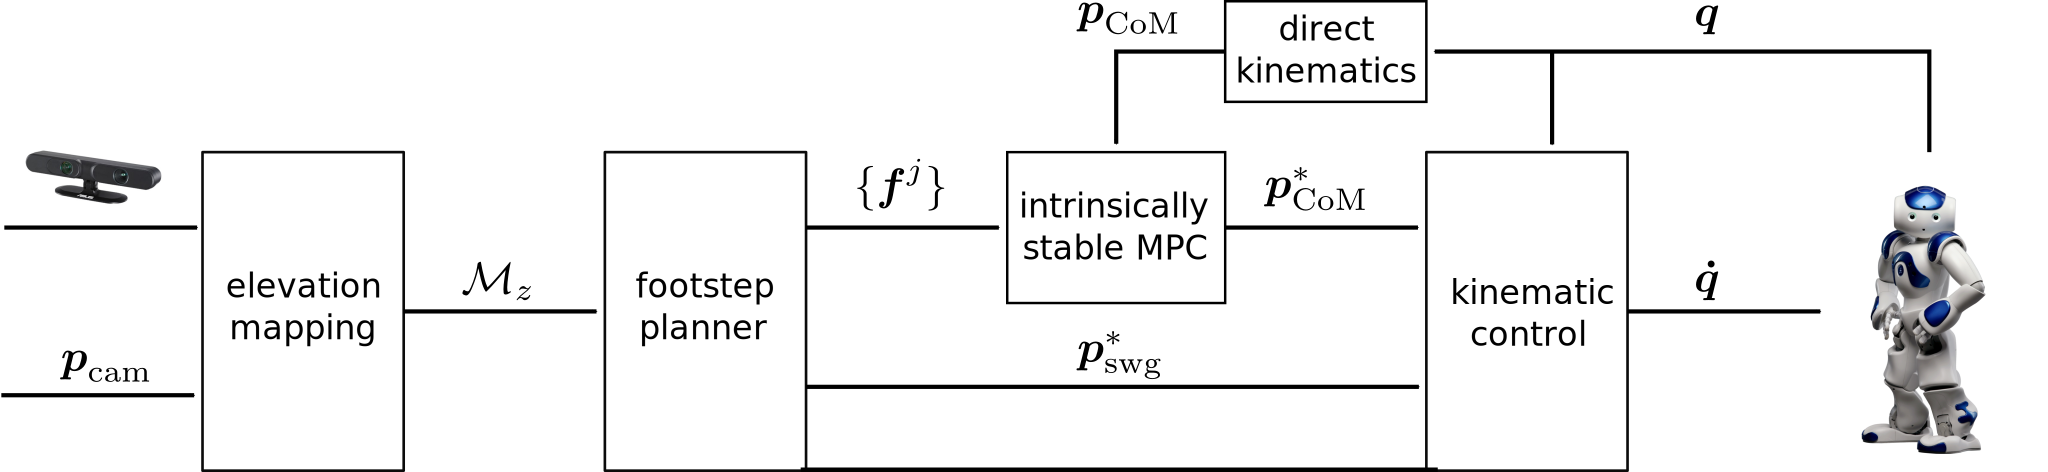
\includegraphics[width=\textwidth]{figures/BlockScheme.pdf}
  \caption{Block scheme of the approach.}
  \label{fig:block-scheme}
\end{figure}

